

\section{Pertoken Dynamics of Benign Fine-tuning}
\label{appendix:dynamics-of-benign-fine-tuning}

This section supplements the analysis of the pertoken dynamics of benign fine-tuning, following the analysis on harmful fine-tuning attacks in Section~\ref{subsubsec:finetuning_stage_vulnerabilities}.

\begin{wrapfigure}{l}{0.41\textwidth}
 \vspace{-2.0em}
 \begin{center}
 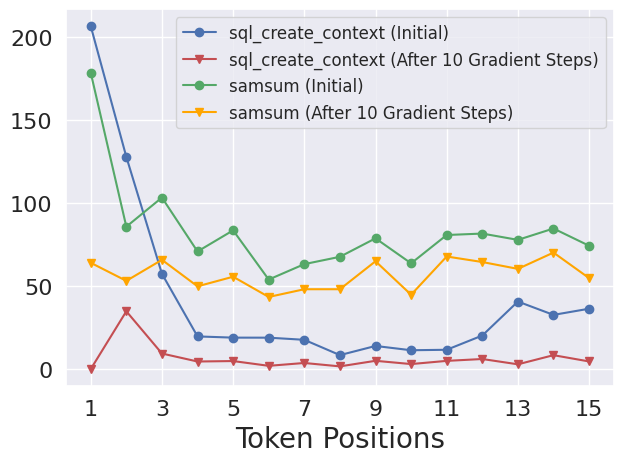
\includegraphics[width=\linewidth]{figs/benign_gradient.png}
 \end{center}
 \vspace{-1em}
 \caption{Per-token Gradient Norm When Fine-tuning Llama-2-7B-Chat on Benign Downstream Tasks Datasets. \textit{Note: 1) ASR of initially aligned model = \underline{$1.5\%$}; 2) After 10 gradient steps on SQL Create Context} = \underline{$13.6\%$}; 3) After 10 gradient steps on Samsum = \underline{$22.1\%$}.}
 \vspace{-1em}
 \label{fig:benign_gradient}
 \end{wrapfigure} 
 
 Interestingly, in addition to fine-tuning attacks where the fine-tuning datasets are intentionally designed to be harmful, {we also note similar per-token dynamics (as in Figure~\ref{fig:pure_bad_per_token_dynamics}) even in purely benign downstream fine-tuning cases.} 
 Figure~\ref{fig:benign_gradient} plots the gradient norm when fine-tuning Llama-2-7B-Chat on SQL Create Context~\cite{b-mc2_2023_sql-create-context} and Samsum~\cite{samsum}. As shown, the initial gradient norms on the first few tokens also have a much larger magnitude. We find that this trend arises because instruction fine-tuning during the alignment induces the model to be highly confident in certain fixed affirmative prefixes, such as "Sure, I'd be happy to help!" on normal inputs. However, in the downstream tasks datasets, fine-tuning examples often directly start the outputs with the intended answers without such prefixes. Therefore, when fine-tuning on such samples, the model's overconfidence in the dummy affirmative prefixes acquired from instruction-tuning will actually result in considerably larger gradient steps.



We hypothesize that \textbf{this might be one underlying reason why \citet{qi2023fine} discover that even benign fine-tuning can cause safety regression in the aligned LLMs} --- it may merely result from the excessively larger gradient steps when updating the generative distributions of these initial transition tokens, which, in turn, lead to over-generalization~(or catastrophic forgetting), and therefore unintendedly also disrupt the model's generative distribution for refusal prefixes in these token positions. This is plausible, as we note that a full fine-tuning on SQL Create Context and Samsum with more than 600 gradient steps results in an increase of ASR from $1.5\%$ to 14.9\% and 25.5\% respectively, but the ASR is already at 13.6\% and 22.1\% after the initial 10 gradient steps. This suggests that the most significant safety regression exactly occurs during these early steps when the gradient norm for the initial tokens is excessively large.
 
